% Chapter Template

\chapter{Large Hadron Collider} % Main chapter title

\label{Chapter3} % Change X to a consecutive number; for referencing this chapter elsewhere, use \ref{ChapterX}

\lhead{Chapter 3. \emph{Large Hadron Collider}} % Change X to a consecutive number; this is for the header on each page - perhaps a shortened title


Physics goals go here.

%----------------------------------------------------------------------------------------
%	SECTION 1
%----------------------------------------------------------------------------------------

\section{Design of the Large Hadron Collider}


\begin{figure}[htbp]
	\centering
		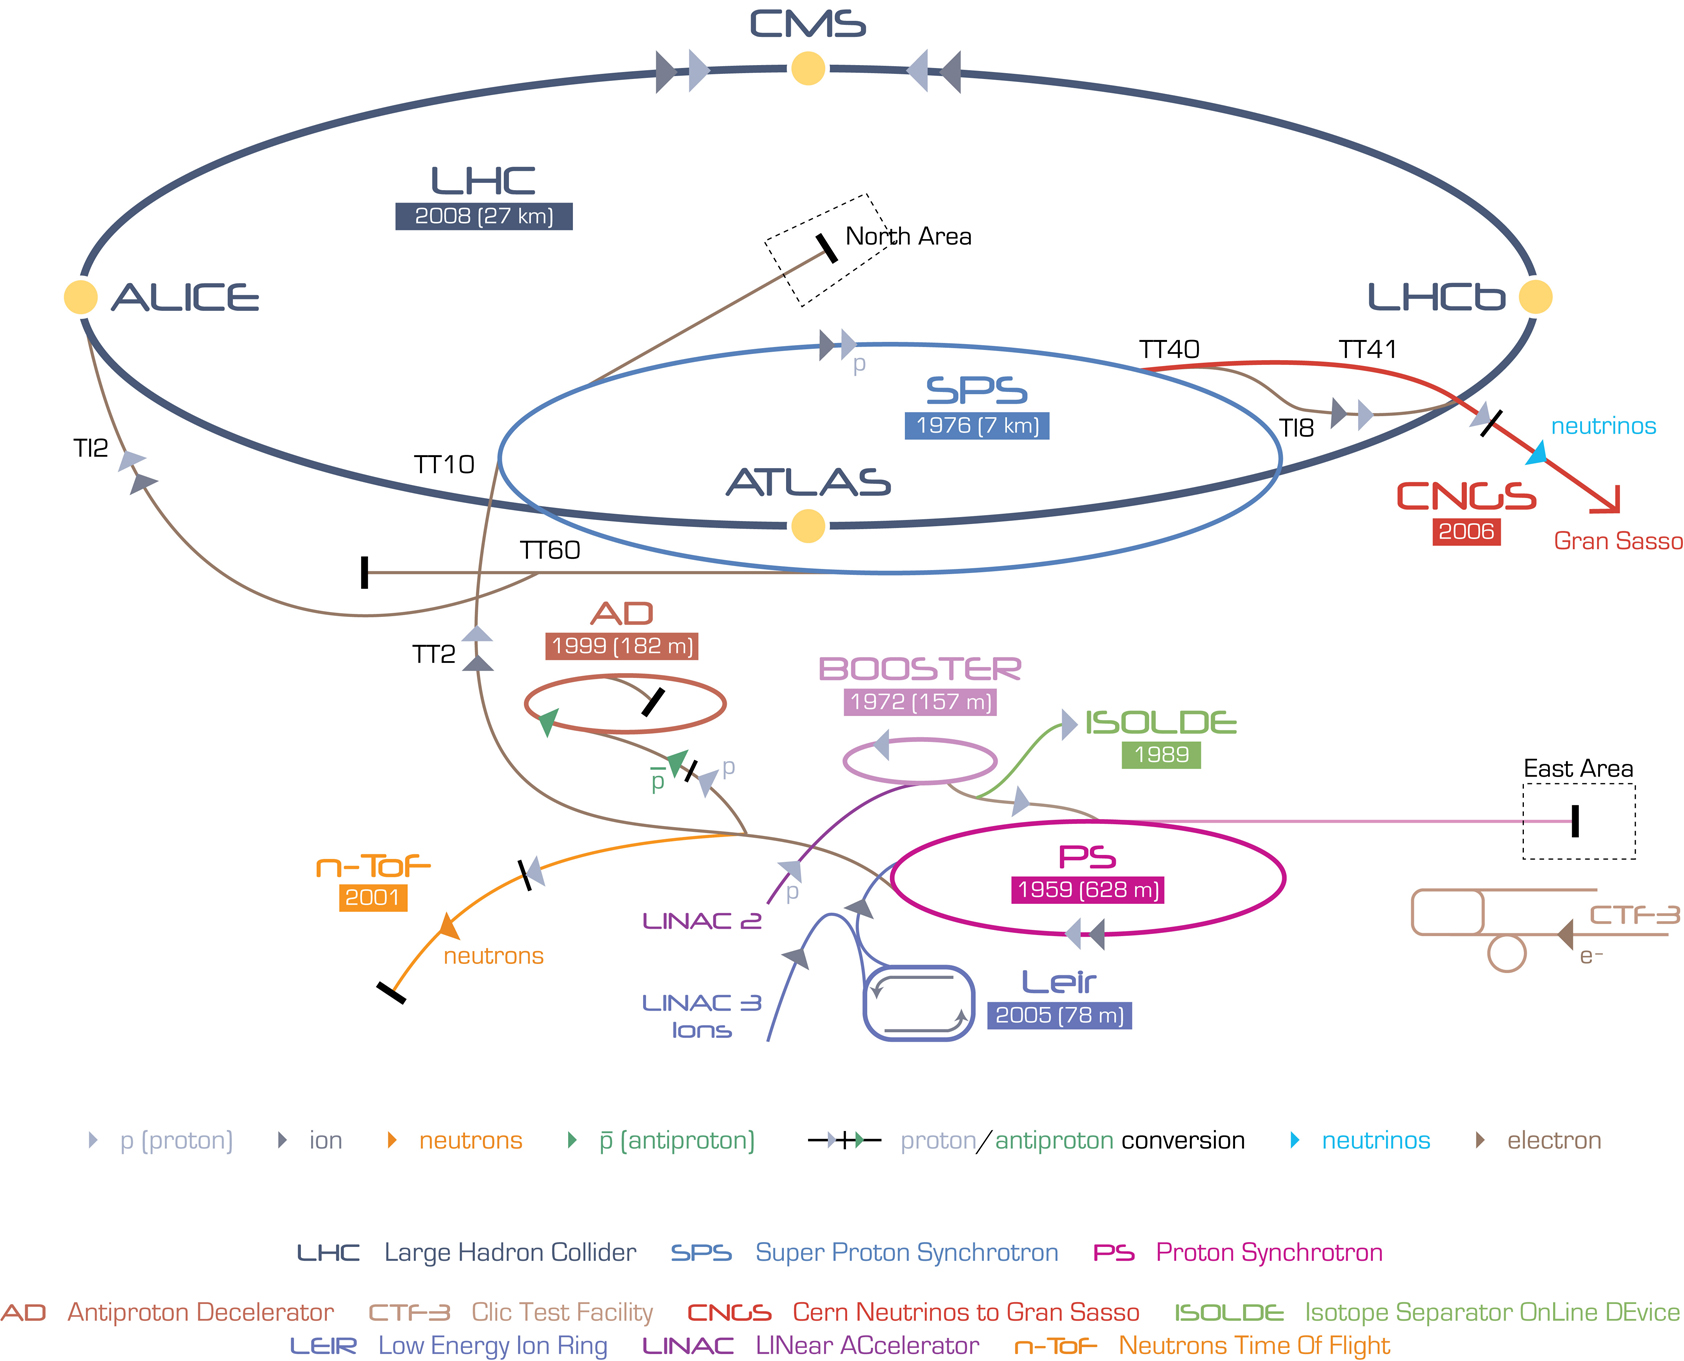
\includegraphics[width=0.8\textwidth]{Figures/LHC.jpg}
		%\rule{35em}{0.5pt}
	\caption[Schematics of Large Hadron Collider]{Schematics of Large Hadron Collider}
	\label{fig:LHC}
\end{figure}

\begin{figure}[htbp]
	\centering
		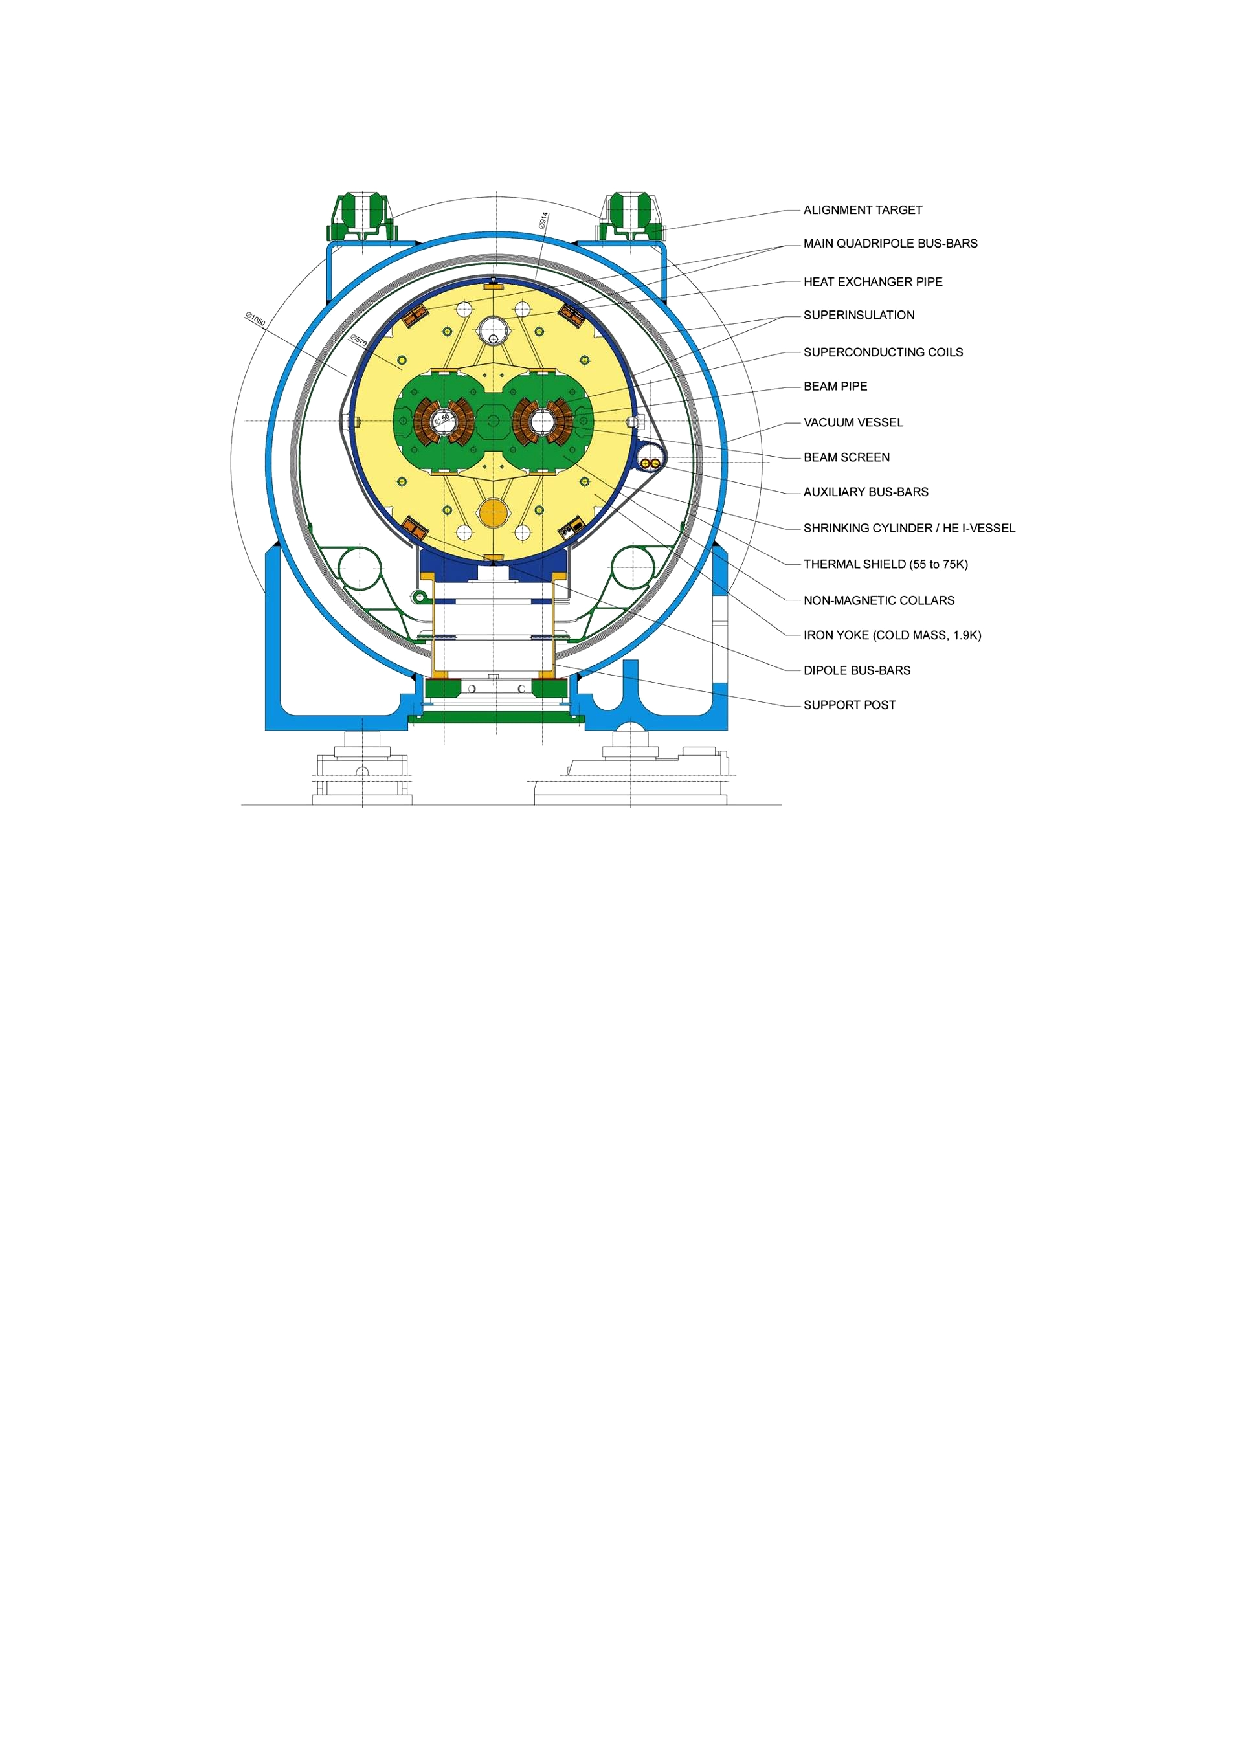
\includegraphics[width=0.7\textwidth]{Figures/LHC_magnet.pdf}
		%\rule{35em}{0.5pt}
	\caption[Schematics of dipole magnets]{Schematics of Dipole magnets}
	\label{fig:LHC_mag}
\end{figure}

%-----------------------------------
%	SECTION 2
%-----------------------------------

\section{Performance}

Since the start of the LHC in 2009, there were three years of machine operation, which yielded many physics results among which the discovery of Higgs boson reported by ATLAS and CMS collaborations. should be highlighted. First year of operation was devoted to commissioning and understanding machine characteristics with the emphasis on safety and testing machine protection systems. In 2011 new energy and instantaneous luminosity records were reached. These numbers were increased once again in 2012 with center of mass energy going to 8 TeV.
\par High bunch intensity with 50 ns bunch spacing was used in order to get a good instantaneous luminosity performance. This came at a cost of high number of collisions in one bunch crossing (pile-up) which was in 2012 around 12 collisions, and in some cases this number went as high as 20 interactions. With the increase of instantaneous luminosity in 2012, number of pile-up interactions was on the average around 30. Besides proton-proton collisions, LHC successfully delivered lead-lead ion runs in 2010 and 2011. primarily for the ALICE experiment, but also for CMS and ATLAS. At the start of 2013. there was also a successful proton-lead run performed for the first time. 

\begin{table}[h]
\centering
  \caption{LHC performance in 2012}
  \begin{tabular}{ l  c  c }
      \hline
      \hline
      Parameter & Design value & Value in 2012 \\
      \hline
      Beam energy [TeV] & 7 & 4 \\
      Bunch spacing [ns] & 25 & 50 \\
      Number of bunches & 2808 & 1374 \\
      Protons per bunch & 1.15$\times 10^{11}$ & 1.6-1.7$\times 10^{11}$ \\
      Peak luminosity [cm$^{-2}$s$^{-1}$] & 1$\times 10^{34}$ & 7.7$\times 10^{33}$ \\
      Max. number of events per bunch crossing & 19 & $\approx 40$ \\
      Stored beam energy [MJ] & 362 & $\approx$ 140 \\
      \hline
      \hline 
  \end{tabular}
\end{table}

LHC head achieved very good luminosity performance during pat years mainly because of the excellent beam quality delivered by the injectors with significantly more protons than nominal and with lower emittances. Since the LHC was capable to absorb these beams, it was chosen to continue to operate with 50 ns bunch spacing. This meant higher pile-up which had to be dealt with by the experiments. 


\begin{table}[h]
\centering
  \caption{LHC performance highlights}
  \begin{tabular}{ l  c }
      \hline
      \hline
      Max. luminosity delivered in one fill & 237 pb$^{-1}$  \\
      Max. luminosity delivered in 7 days & 1.35 fb$^{-1}$  \\
      Longest time in stable beams (2012) & 22.8 hours \\
      Longest time in stable beams over 7 days & 91.8 hours (55$\%$) \\
      \hline
      \hline 
  \end{tabular}
\end{table}

\begin{figure}[htbp]
	\centering
		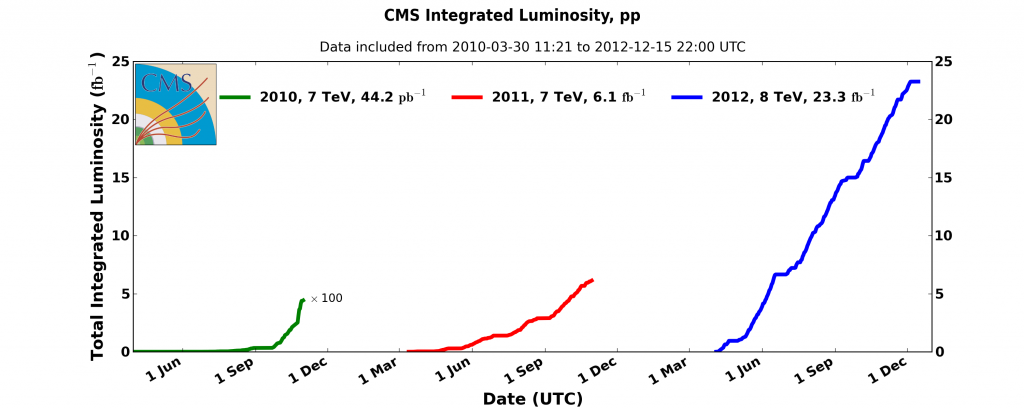
\includegraphics[width=0.7\textwidth]{Figures/lumi.png}
		%\rule{35em}{0.5pt}
	\caption[Luminosity delivered to the CMS experiment]{Luminosity delivered to the CMS experiment}
	\label{fig:LHC_lumi}
\end{figure}
 
Following a two year shutdown, LHC is anticipating operations at even higher energies of 6.5 TeV and later 7 TeV. The long term plan includes even higher peak luminosities, installation of the new injector complex and later the beginning of HL-LHC era. The timeline will, of course, be highly affected by the performance and results of the next run.